
\begin{figure}
    \centering
    \includegraphics[width=\textwidth,trim={0 2cm 0 0},clip]{../Figures/flat/SI1_Human.jpg}
    \captionof{figure}{\textbf{Color categories assessed in human participants with a nonverbal paradigm. }
    Prior work by \citep{bae_why_2015} and \citep{panichello_error-correcting_2019} has used a task in which participants match the color of a cue to a continuous ring of colors; those published results were obtained with a combination of in-person experiments and on-line experiments, and the results are consistent for both kinds of experiments. 
    A mixture-model analysis of the results recovers four color categories, corresponding to blue, green, orange and pink. 
    Note that the data from \citep{bae_why_2015} shown in the figure were from just three participants; those authors confirmed the results in more subjects with a version of the task that omitted the memory delay period (so the cue and the match-option color wheel were presented simultaneously). 
    The present work adapted the paradigm so that the match options were discrete targets, which avoids the risk of reinforcing idiosyncratic biases that arises when using the task in non-human primates, by allowing greater precision (only direct matches are rewarded). 
    In human participants, with experiments conducted online with Amazon Mechanical Turk, the results using the discrete-matching paradigm recover the same number of significant color categories as the continuous-matching paradigm.
    These four categories correspond to the four categories recovered in the prior work, blue, green, orange, pink. 
    We note that the discrete-matching task recovers a trend for a fifth category that would correspond to “purple”; close inspection of the results in Bae et al (2015) also provide evidence of this trend. 
    } 
    \label{fig:Human}
\end{figure}



% \begin{appendixbox}
%         \includegraphics[width=\textwidth]{../Figures/flat/SI2_psychometric.jpg}
%         \captionof{figure}{\textbf{foo}
%         \emph{a} test
%         } 
%         \label{fig:IndiDiff}
% \end{appendixbox}

% \begin{appendixbox}
%         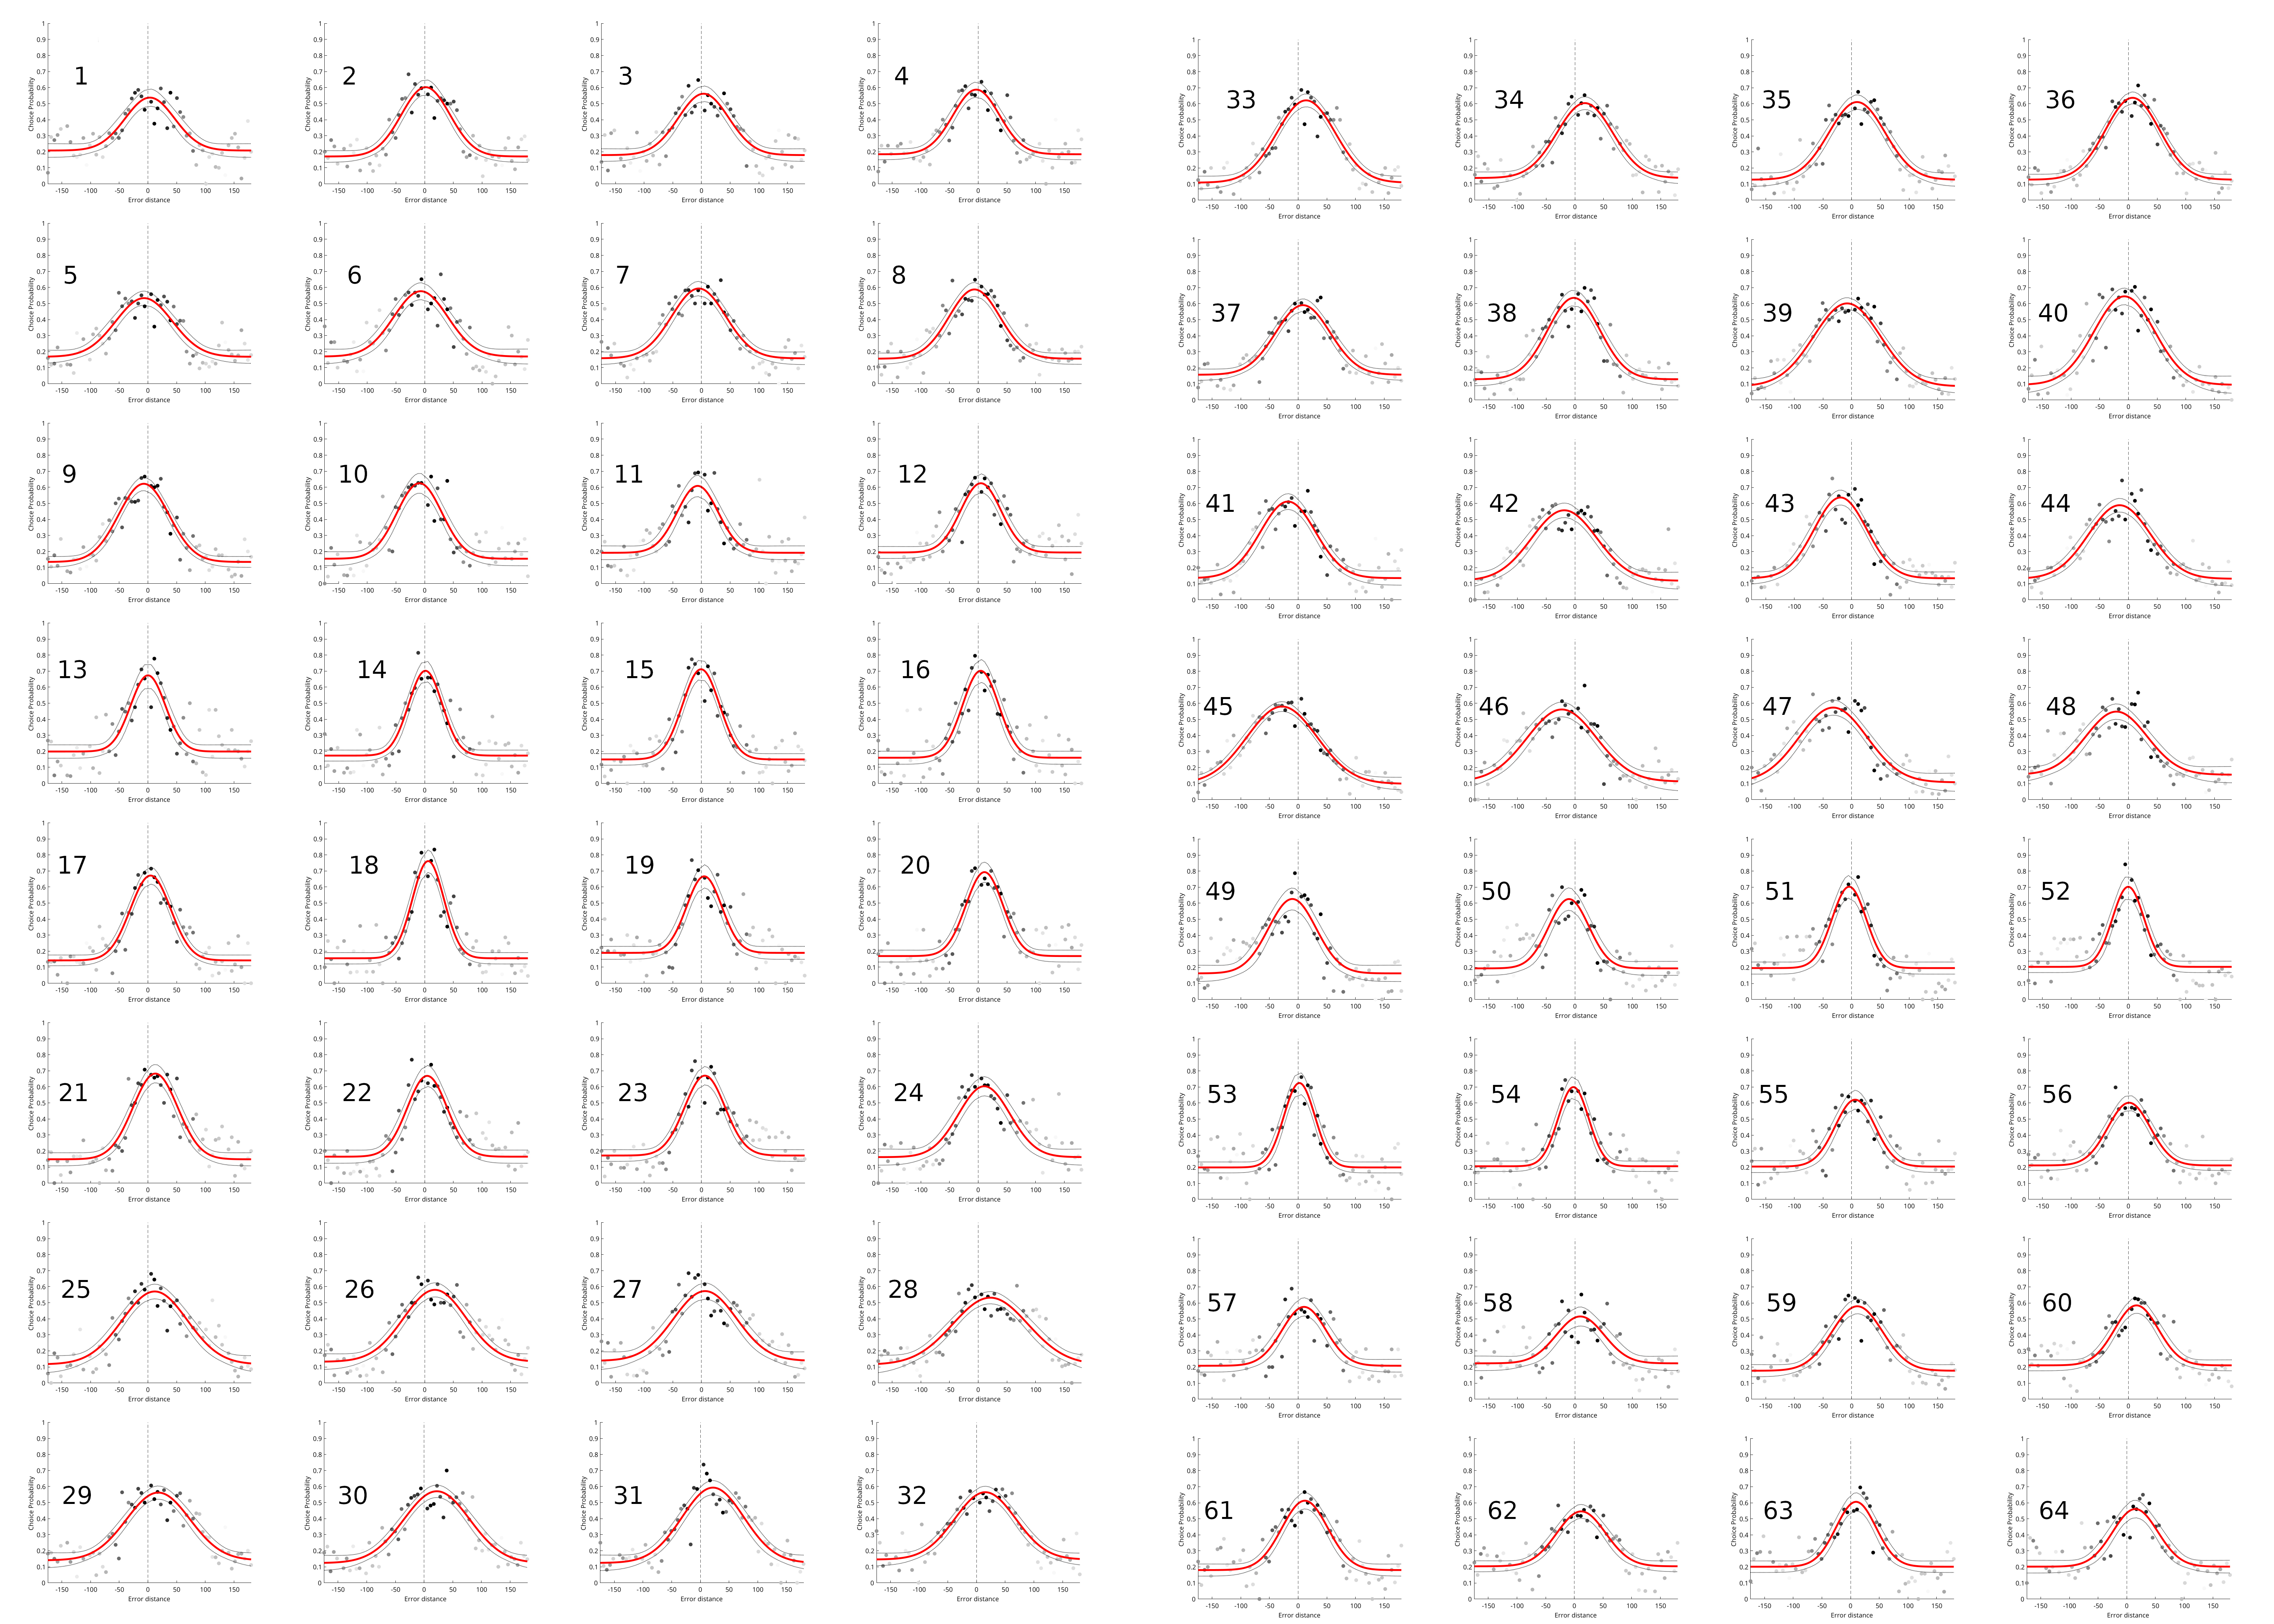
\includegraphics[width=\textwidth]{../Figures/flat/SI3_MMBreakOut.jpg}
%         \captionof{figure}{\textbf{foo}
%         \emph{a} test
%         } 
%         \label{fig:MMBreakOut}
% \end{appendixbox}

% \begin{appendixbox}
%         \includegraphics[width=\textwidth]{../Figures/flat/SI4_MM.jpg}
%         \captionof{figure}{\textbf{foo}
%         \emph{a} test
%         } 
%         \label{fig:MM}
% \end{appendixbox}

% \begin{appendixbox}
%         \includegraphics[width=\textwidth]{../Figures/flat/SI5_IndTCCv.jpg}
%         \captionof{figure}{\textbf{foo}
%         \emph{a} test
%         } 
%         \label{fig:IndiTCC}
% \end{appendixbox}

% \begin{appendixbox}
%         \includegraphics[width=\textwidth]{../Figures/flat/SI6_choiceMatrices.jpg}
%         \captionof{figure}{\textbf{foo}
%         \emph{a} test
%         } 
%         \label{fig:choiceProbabilityMatrices}
% \end{appendixbox}

